\chapter{Background}
\label{chap:background}

This chapter outlines the fundamental concepts and technologies that underpin the system's design and implementation. It includes an overview of the hardware platforms used for embedded development, the cryptographic mechanisms for securing data, the principles of NFC communication, and the prototyping and communication protocols that enable interaction between components.

\section{Embedded Hardware and Development Environment}
\label{sec:embedded_hw}

The objective of this section is to describe the embedded platforms used for the development of the prototype. These solutions provide an accessible programming environment and a large support community, which facilitates iterative hardware implementation and the incorporation of specialized libraries.

\subsection{Arduino}
\label{subsec:arduino}
Arduino is an open-source software and hardware platform based on a board that includes electronic circuits with analog and digital inputs and outputs.  
The first Arduino board was introduced in 2005, and its popularity has not yet started to decrease.

One of the main reasons for this reputation is the wide number of modules it is compatible with, which leads to great flexibility in educational projects related to robotics and automation.

Arduino boards are small, low-power consuming computers. As shown in Figure~\ref{fig:arduino}, they have several components with different functionalities~\cite{Ref8}:

\begin{itemize}
	\item \textbf{Microcontroller:} receives and sends information to the devices connected to it. The specific chip depends on the board model.
	\item \textbf{External power supply:} powers the microcontroller with a DC voltage range of 9--12V.
	\item \textbf{USB plug:} used to upload code to the microcontroller through a USB cable. It can also supply 5V DC in absence of external power.
	\item \textbf{Internal programmer}
	\item \textbf{Reset button}
	\item \textbf{Analog pins:} used for analog input/output. Quantity varies between models.
	\item \textbf{Digital pins:} used for digital input/output. Quantity also varies.
	\item \textbf{Power and GND pins:} provide 3.3V, 5V and ground connections.
\end{itemize}
The board used in this project is an \textit{Arduino Uno}, which uses an ATmega328 microcontroller, has a clock speed of 16\,MHz with auto-reset, 14 digital I/O pins, 6 analog inputs, USB-B connection, and 32\,KB flash memory.  
The key feature regarding the selection of this board was the wide documentation available online~\cite{Ref9}.

\begin{figure}[h!]
	\centering
	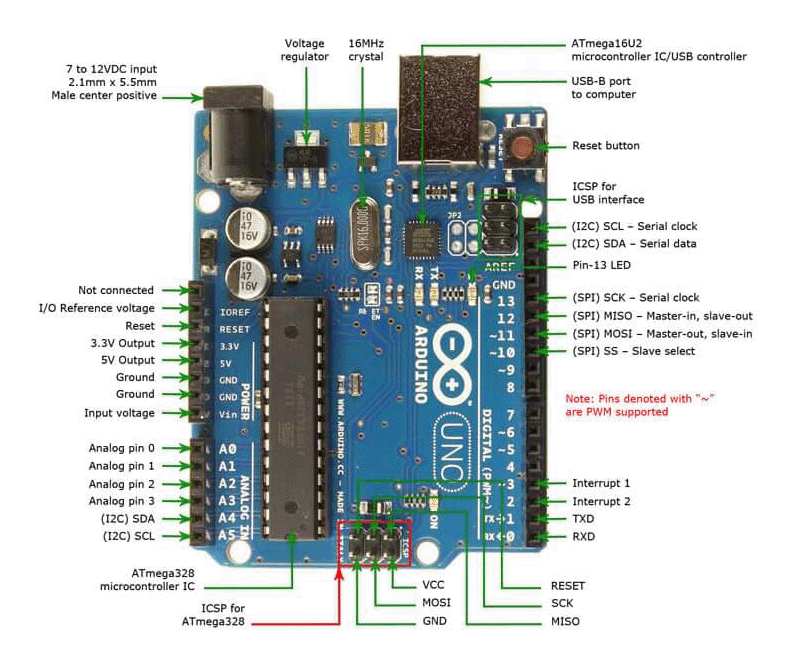
\includegraphics[width=0.65\textwidth]{imaxes/arduino-pinout.png}
	\caption{Connectivity diagram of Arduino UNO hardware development board}
	\label{fig:arduino}
\end{figure}

Arduino provides an IDE, which is a simplified integrated platform that helps users to develop software code efficiently using the C or C++ programming languages. The code written for the Arduino board is called a \textit{sketch}.

Arduino programming language is designed to be accessible and intuitive. It has several built-in functions.

There are two main functions that must be present in all sketches:

\begin{itemize}
	\item \texttt{void setup()}: first process run when Arduino starts. It runs once. Pin modes must be declared here.
	\item \texttt{void loop()}: this code will run endlessly.
\end{itemize}

Other commonly used predefined functions include:

\begin{itemize}
	\item \texttt{digitalWrite(pin, HIGH/LOW)}: sets the digital pin N state to HIGH (5V) or LOW (0V).
	\item \texttt{digitalRead(pin)}: : reads the value from a specified digital pin, either HIGH or
	LOW.
	\item \texttt{analogWrite(pin, value)}: writes an analog value to a pin.
	\item \texttt{analogRead(pin)}: reads the value of an analog pin.
\end{itemize}

There are predefined and third-party libraries that simplify the integration of specific
hardware and modules, such as NFC, WiFi and Bluetooth. These libraries
encapsulate advanced functionalities, reducing development complexity~\cite{Ref10}.

\subsection{ESP32}
\label{subsec:esp32}


The ESP32 is a low-cost, low-power microcontroller designed by Espressif Systems, mainly oriented to Internet of Things (IoT) applications. It is a versatile solution that combines Wi-Fi and Bluetooth connectivity in a single chip, allowing its integration in projects that require wireless communication, device control, and real-time data transmission~\cite{Ref11}.

One of the main features of ESP32 are:

\begin{itemize}
	\item \textbf{Processor:} Xtensa LX6 dual-core operating at
	frequencies up to 240 MHz.
	\item \textbf{Memory:} 520 KB of SRAM and support for up to 16 MB of external flash
	memory.
	\item \textbf{Connectivity:} Wi-Fi (802.11 b/g/n), Bluetooth 4.2 (BLE and BR/EDR).
	\item \textbf{Input/Output interfaces:}  Up to 32 multifunction GPIO pins, support for
	protocols such as UART, SPI, I2C, PWM, ADC (12 bits) and DAC (8 bits).
	\item \textbf{Compatibility with Libraries and Tools::}  Programmable using the ESP-IDF
	development framework or more accessible platforms such as Arduino IDE.
	Compatible with languages such as C/C++ and frameworks such as
	FreeRTOS for real-time applications.
\end{itemize}

\begin{figure}[h!]
	\centering
	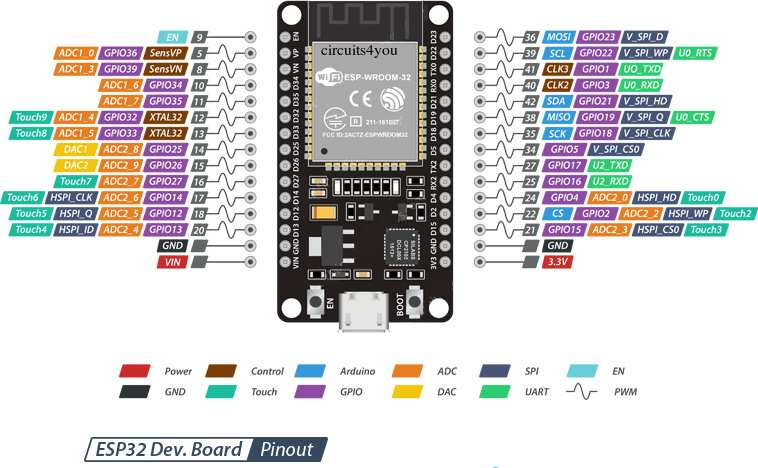
\includegraphics[width=0.8\textwidth]{imaxes/ESP32-Pinout.jpg}
	\caption{Connectivity diagram of ESP32 hardware development board}
	\label{fig:esp32}
\end{figure}






\subsection{Protoboard}
\label{subsec:protoboard}

For the design and testing of electronic circuits in the system, \textit{Protoboard}, also
known as breadboard, was chosen as the most appropriate tool for this purpose. It is
a rectangular plastic board containing an array of slots interrelated with thin plates of
copper, which though are internally connected within the board, also matting with
any electronic component without soldering it permanently. The central columns are
usually divided by a slot, separating two independent sections. Each column of five
holes is internally connected, facilitating the insertion of components and their
interconnection. To connect components together, their pins must be inserted into
the same column or cables must be used to connect different columns \cite{Ref14}.

The main purpose of a breadboard is to help easy and fast prototyping of the circuits,
so that the designer or students can assemble, reconfigure and test
different combinations quickly. The ability to create temporary connections on an
as-needed basis can be particularly helpful during the early stages of development,
where it is often necessary to make tweaks and optimizations to the design of a
given circuit. Also, its modular and reusable design renders it invaluable in both
academic and industrial settings.




\clearpage

\section{Cryptographic Mechanisms for NFC-Based Access Control}
\label{sec:crypto_mechs}
This section presents cryptographic mechanisms used to guarantee the confidentiality, integrity and authenticity of communications in access control systems.


\subsection{AES-128}
\label{subsec:aes128}

AES-128 is a symmetric encryption algorithm that uses a 128-bit key to protect data confidentiality and integrity. Its robust and efficient design makes it ideal for NFC-based access control systems.

During the AES-128 Encryption Process, a 128-bit block of data is taken along with a 128-bit key as input. The cipher goes through 10 rounds of transformations:

\begin{itemize}
	\item \textbf{Substitution (SubBytes):} Each byte is replaced by another byte using a substitution table (S-Box).
	\item \textbf{Shift (ShiftRows):} The bytes in the rows of the block are rearranged.
	\item \textbf{MixColumns:} The columns are combined to spread the data.
	\item \textbf{AddRoundKey:} Each round is combined with a key derived from the original.
\end{itemize}

Finally, the output is a 128-bit encrypted block of data. The receiver decrypts the data using the same key, ensuring that only authorized parties can access the information. The decryption process is the same as the encryption but reversing the order of the transformations~\cite{Ref12}.

\begin{figure}[H]
	\centering
	\includegraphics[width=0.7\textwidth]{imaxes/aes-128.png}
	\caption{AES-128 Encryption Process, including Substitution, Shift, MixColumns, and AddRoundKey}
	\label{fig:aes128}
\end{figure}


\subsection{HMAC-SHA256}
\label{subsec:hmac}

HMAC stands for \textit{Hash-based Message Authentication Code}. It is a cryptographic mechanism that ensures data integrity and authenticity by combining a cryptographic hash function with a shared secret key. Its purpose is to prevent unauthorized modification of transmitted messages and to verify the identity of the sender.

HMAC is meant to use a standard hash function, such as SHA-256, in combination with a secret key to generate an authentication code. If the key is longer than the block size of the hash function (64 bytes for SHA-256), it is truncated by applying the hash function; if it is shorter than 64 bytes, it is padded with zeroes.

An inner key is obtained by combining the key with a fill value called \texttt{ipad} (0x36 repeated). In addition, an outer key is obtained by combining the key with a fill value called \texttt{opad} (0x5C repeated).

The hash function is applied on the concatenation of the inner key and the message.  
Then, the algorithm is applied again on the concatenation of the outer key and the result obtained in the previous step. The whole equation applied is:

\[
\text{HMAC}(K,M) = H\big((K \oplus \text{opad}) \parallel H((K \oplus \text{ipad}) \parallel M)\big)
\]

where $K$ is the secret key, $M$ is the message, $H$ is the hash function, $\oplus$ represents the XOR operation, and $\parallel$ indicates concatenation~\cite{Ref21}.

MAC provides collision resistance, which takes advantage of the properties of the
underlying hash function, reducing the probability of two different messages
producing the same HMAC code. Also, it ensures protection against length extension
attacks, because the message is processed within a structure with a secret key
before the final application of the hash function, hash extension attacks are
mitigated.


\subsection{Hardware Security Module (HSM)}
\label{subsec:hsm}

A Hardware Security Module (HSM) is a dedicated, tamper-resistant piece of
hardware designed to generate, store and use cryptographic keys in a way that
keeps them isolated from potentially compromised general-purpose systems. In
essence, an HSM provides a “vault” for the most sensitive secrets (root keys,
certificate‐signing keys, master passwords, etc.) and enforces that any
cryptographic operation involving those keys happens entirely inside the module~\cite{Ref22}.

There are different types of HSM:

\paragraph{Physical HSM:}
\begin{itemize}
	\item Typically rack-mountable appliances that sit in a data-center.
	\item They connect to host systems over a secure network or PCIe interface and expose a well-defined API (such as PKCS\#11) for requesting cryptographic operations.
	\item Internally combine high-grade CPUs, hardware random-number generators, and physical tamper-sensors (which erase keys on attack).
\end{itemize}

\paragraph{Network-attached (or “cloud”) HSMs:}
\begin{itemize}
	\item Functionally very similar to physical HSMs, but located in a cloud provider’s data centers.
	\item Access is mediated via secure, often RESTful, APIs.
	\item Provide turnkey elasticity and geo-redundancy, but trust is required in the cloud vendor’s physical and personnel security.
\end{itemize}

\paragraph{Virtual HSMs (vHSMs):}
\begin{itemize}
	\item Software-only implementations that pretend to offer an HSM interface.
	\item Rely on software isolation (e.g., VMs or containers) rather than true hardware separation.
	\item Lighter weight and cheaper, but cannot guarantee the same level of protection against a compromised host.
\end{itemize}

\paragraph{Hybrid approaches:}
\begin{itemize}
	\item Embed a minimal “root” HSM in hardware or a vendor-provided trusted execution environment (e.g., TPM or ARM TrustZone), which in turn “unlocks” a software vHSM for day-to-day operations.
	\item Balances cost versus security: the hardware root protects the long-term keys, while the vHSM handles high-volume crypto.
\end{itemize}

\section{NFC}
\label{sec:nfc}

Near Field Communication (NFC) is a short-range wireless communication technology that enables data transfer between devices at a typical distance of 4 to 10 cm in non critical applications \cite{ref63} and $\geq 4$ cm in secure based applications \cite{ref64}. It is used in authentication and access control systems because of its security, ease of use and low power consumption. Thus, NFC systems are actually part of RFID technology, i.e. they can be considered as a subgroup within RFID techniques.

NFC uses an electromagnetic field to establish a connection between a reader device (active) and a tag device (passive). Data is transferred using secure protocols, following standards such as ISO/IEC 14443 \cite{Ref2}. Also, its limited range significantly reduces the risk of data interception.

NFC devices can operate in two modes:

\begin{itemize}
	\item \textbf{Reader/Writer:} The active device reads or writes data to the NFC tag.
	\item \textbf{Card Emulation:} An NFC device acts as a tag to be read by a reader.
\end{itemize}


\subsection{NFC UID}
\label{subsec:nfc_uid}

The UID (Unique Identifier) is a unique identifier assigned to each NFC tag, mainly used to uniquely identify each device in a system. This identifier can be static or dynamic, depending on the specifications of the NFC tag.

Static UID is the most common; it is immutable and serves as a unique identifier to validate access in simple systems. However, its ease of cloning represents a security risk in critical systems. On the other hand, dynamic UID is temporarily generated or variable at each interaction, it is usually encrypted and is much more secure than the static UID \cite{ref13}. It is used in advanced NFC cards and access systems that prioritize protection against attacks such as impersonation or cloning.


\subsection{MFRC522}
\label{subsec:mfrc522}

The MFRC522 module is an RFID/NFC reader/writer, which is based on NFC technology used for authentication and contactless payments at 13.56 MHz frequency. Its versatility and low cost made it a popular choice for many access control, electronic payment and inventory management applications. In addition, it supports ISO/IEC 14443A (MIFARE Classic, Ultralight and NTAG authentication). Its typical communication range is 1 to 3 cm, making it suitable for secure applications where physical proximity is required for authentication \cite{Ref15}.

Its low power consumption makes it ideal for embedded devices such as Arduino. Also, it includes a flexible communication interface compatible with different microcontrollers and communication protocols (SPI, I2C, UART). Security is provided through authentication with access keys in memory sectors, protecting the integrity of the data stored on the card. In addition its writing and reading capability allows the storage of information such as unique identifiers or balances in payment cards.

